        \clearpage
        \begin{figure*}[ht]
            \pdfbookmark[2]{ID 01}{figure_id_01}
        	\centering
            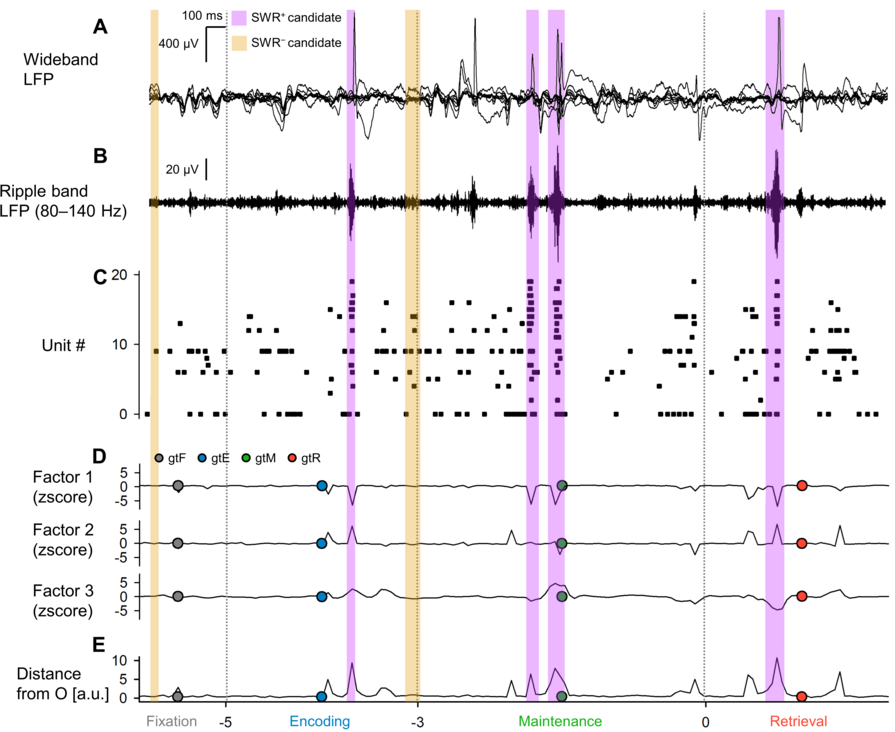
\includegraphics[width=1\textwidth]{./src/figures/.png/Figure_ID_01.png}
        	\caption{\textbf{Local Field Potential (LFP), Multiunit Activity, and Neural Trajectory of the Hippocampus during a Modified Sternberg Task} \cite{li_functional_2023, borders_hippocampal_2022, dimakopoulos_information_2022}}
\smallskip
\\
\textbf{\textit{A.}} This segment presents representative wideband LFP traces from iEEG signals, observed in the left hippocampal head throughout the completion of a modified Sternberg working memory task. The task involves fixation (1 s, \textit{gray}), encoding (2 s, \textit{blue}), maintenance (3 s, \textit{green}), and retrieval (2 s, \textit{red}) \cite{li_functional_2023, borders_hippocampal_2022, dimakopoulos_information_2022}. \textbf{\textit{B.}} The corresponding ripple band LFP traces are depicted here \cite{schomburg_spiking_2012, behrens_induction_2005, norimoto_hippocampal_2018}. \textbf{\textit{C.}} The raster plot of multiunit spikes, derived from the LFP traces utilizing a spike sorting algorithm, is illustrated here \cite{niediek_reliable_2016}. \textbf{\textit{D.}} This part represents the neural trajectory, established by the GPFA, computed from the spike counts per unit within 50-ms bins \cite{yu_gaussian-process_2009}. The dotted circles represent the geometric median coordinates for each phase. \textbf{\textit{E.}} The distance from the trajectory to the point $O$ is demonstrated here. It is notable that the \textit{purple} and \textit{yellow} rectangles denote the timings for SWR$^+$ candidates and SWR$^-$ candidates, respectively, functioning as controls for SWR$^+$ \cite{van_vugt_hippocampal_2010, scoville_loss_1957, kay_hippocampal_2016, nader_memory_2003, wilson_reactivation_1994, nadasdy_replay_1999, lee_memory_2002}.
}
% width=1\textwidth
        	\label{fig:01}
        \end{figure*}
